\documentclass{sig-alternate}
\usepackage{graphicx}
\usepackage{latexsym}
\usepackage{hyperref}
\usepackage{amsmath}
\usepackage{float}
\usepackage{xspace}
\usepackage{epstopdf}
\usepackage{hhline}
%\usepackage{algorithm}
%\usepackage{algorithmic}
%\usepackage{algorithmwh}
\usepackage[vlined,ruled]{algorithm2e}
%\SetAlFnt{\small}
%\SetAlCapFnt{\small}


\usepackage{amssymb}
\usepackage{subfigure}


\usepackage{lipsum}
\usepackage{paralist}
\usepackage{fixmath}
\usepackage{rotating}
\usepackage{listings}
\usepackage{booktabs}
\usepackage{threeparttable}
\usepackage{multirow}
\usepackage{array}

\usepackage{enumitem}
\usepackage{balance}


\usepackage{color}

\usepackage{textcomp}

\definecolor{listinggray}{gray}{0.9}
\definecolor{lbcolor}{rgb}{0.9,0.9,0.9}
\lstset{
	%backgroundcolor=\color{lbcolor},
	tabsize=2,
	rulecolor=,
	language=html,
        basicstyle=\scriptsize,
        upquote=true,
        aboveskip={0.5\baselineskip},
        columns=fixed,
        showstringspaces=false,
        extendedchars=true,
        breaklines=true,
        prebreak = \raisebox{0ex}[0ex][0ex]{\ensuremath{\hookleftarrow}},
        frame=single,
        showtabs=false,
        showspaces=false,
        showstringspaces=false,
        identifierstyle=\ttfamily,
        keywordstyle=\color[rgb]{0,0,1},
        commentstyle=\color[rgb]{0.133,0.545,0.133},
        stringstyle=\color[rgb]{0.627,0.126,0.941},
        %emphstyle=\color[rgb]{0.827,0.126,0.941},
}


%Listings for JS
\definecolor{lightgray}{rgb}{.9,.9,.9}
\definecolor{darkgray}{rgb}{.4,.4,.4}
\definecolor{purple}{rgb}{0.65, 0.12, 0.82}
\definecolor{forestgreen}{rgb}{0.13, 0.55, 0.13}

\lstdefinelanguage{JavaScript}{
  keywords={typeof, new, true, false, catch, function, return, null, catch, switch, var, if, for, in, while, do, else, case, break, assertEquals, assertTrue,equal, ok},
  keywordstyle=\color{blue}\bfseries,
  ndkeywords={class, export, boolean, throw, implements, import, this, By, int,@Test},
  ndkeywordstyle=\color{darkgray}\bfseries,
  identifierstyle=\color{black},
  sensitive=false,
  comment=[l]{//},
  morecomment=[s]{/*}{*/},
  commentstyle=\color{forestgreen}\ttfamily,
  stringstyle=\color{purple}\ttfamily,
  morestring=[b]',
  morestring=[b]"
}
\lstset{
   language=JavaScript,
   %backgroundcolor=\color{lightgray},
   extendedchars=true,
   basicstyle=\scriptsize\ttfamily,
   showstringspaces=false,
   showspaces=false,
   numbers=left,
   numberstyle=\scriptsize,
   numbersep=-6pt,
   tabsize=2,
   breaklines=true,
   showtabs=false,
   captionpos=b,
   numberblanklines=false
%   escapeinside=\[\]
   }
%\DeclareFontShape{T1}{lmr}{bx}{sc} { <-> ssub * cmr/bx/sc }{}
%\textwidth 17.8cm
%\textheight 22.7cm
%\setstretch{0.95}

%%Terminology
\newcommand{\rest}{\textsc{Rest}\xspace}
\newcommand{\jsf}{\textsc{Jsf}\xspace}
\newcommand{\ajax}{\textsc{Ajax}\xspace}
\newcommand{\headbf}[1]{\par\smallskip\noindent\textbf{#1.}}
\newcommand{\head}[1]{\subsubsection{#1}}
\newcommand{\headed}[1]{\noindent\textbf{#1}\ \ }
\newcommand{\webtwo}{\textit{Web~2.0}\xspace}
\newcommand{\crawljax}{\textsc{Crawljax}\xspace}
\newcommand{\petstore}{\textsc{PetStore}\xspace}
\newcommand{\etal}{et al.\xspace}
\newcommand{\ie}{{i.e.,}\xspace}
\newcommand{\eg}{{e.g.,}\xspace}
\newcommand{\atusatwo}{\textsc{Atusa~2.0}\xspace}
\newcommand{\tudu}{\textsc{TUDU}\xspace}
\newcommand{\todo}{\textsc{Todo}\xspace}
\newcommand{\taskfreak}{\textsc{TaskFreak}\xspace}
\newcommand{\tocview}{\textsc{TocView}\xspace}
\newcommand{\javascript}{Java\-Script\xspace}
\newcommand{\jquery}{\textsc{jQuery}\xspace}
\newcommand{\hitlist}{\textsc{HitList}\xspace}
\newcommand{\googlereader}{\textsc{Google Reader}\xspace}
\newcommand{\testsuite}[1]{\textsc{Test Suite #1}\xspace}
\newcommand{\version}[1]{\textsc{V#1}\xspace}
\newcommand{\proc}[2]{{\textbf{Procedure} \textsc{#1}(\textit{#2})}}

\newcommand{\mutandis}{\textsc{Mutandis}\xspace}
\newcommand{\jsart}{\textsc{JSart}\xspace}
\newcommand{\tool}{\textsc{Atrina}\xspace}
\newcommand{\artemis}{\textsc{Artemis}\xspace}
\newcommand{\qunit}{\textsc{QUnit}\xspace}
\newcommand{\junit}{\textsc{JUnit}\xspace}
\newcommand{\selenium}{\textsc{Selenium}\xspace}
\newcommand{\blanket}{\textsc{Blanket}\xspace}
\newcommand{\jscover}{\textsc{JSCover}\xspace}


\newcommand{\cssparser}{\textsc{CSSParser}\xspace}

\newcommand{\myspace}{\hspace{1mm}}


%% abbreviations and commands
\newcommand{\secref}[1]{Section~\ref{Sec:#1}}
\newcommand{\figref}[1]{Figure~\ref{Fig:#1}}
\newcommand{\listref}[1]{Listing~\ref{List:#1}}
\newcommand{\tabref}[1]{Table~\ref{Table:#1}}
\newcommand{\algref}[1]{Algorithm~\ref{Alg:#1}}
\newcommand{\curl}[1]{\footnote{~\scriptsize\url{#1}}}
\newcommand{\fn}[1]{\footnote{~\scriptsize{#1}}}
\newcommand{\code}[1]{{\texttt{#1}}}
\newtheorem{mydef}{Definition}


\newcommand{\mycaption}[1]{%
%\vspace{-1.3\baselineskip}
\caption{#1}
}

\lstloadlanguages{Java,XML,HTML}



\newcommand{\aff}[1]{{\normalsize \textsl{#1}}}

% TeX hack to make timestamp

%
\def\sharedaffiliation{%
\end{tabular}
\begin{tabular}{c}}
%
 \def\now{{\def\Time{3}\def\Hour{4}\def\Minute{5}%
  \count\Time=\time\relax\ifnum\count\Time=0\count\Time=1440\fi%
  \count\Hour=\count\Time\relax\divide\count\Hour by 60\relax%
  \count\Minute=\count\Hour\relax\multiply\count\Minute by -60\relax%
  \advance\count\Minute by \count\Time\relax\the\count\Hour\relax:%
  \ifnum\count\Minute<10 0 \fi\the\count\Minute\relax}}
  
\newboolean{showcomments}
\setboolean{showcomments}{false}
\ifthenelse{\boolean{showcomments}}
{\newcommand{\nb}[2]{
\fbox{\bfseries\sffamily\scriptsize#1}
{\sf\small$\blacktriangleright$\textit{#2}$\blacktriangleleft$}
}
}
{\newcommand{\nb}[2]{}
}
\newcommand\ali[1]{\nb{Ali}{#1}}
\newcommand\shabnam[1]{\nb{Shabnam}{#1}}
\newcommand\karthik[1]{\nb{Karthik}{#1}}


\newcommand{\theadturn}[1]{%
\begin{turn}{90}\textbf{#1}\end{turn}
}

\newcommand{\thead}[1]{%
\textbf{#1}
}

\newcommand{\footnoteremember}[2]{\footnote{~\scriptsize{#2}}
  \newcounter{#1}
  \setcounter{#1}{\value{footnote}}}
\newcommand{\footnoterecall}[1]{\footnotemark[\value{#1}]
}

% Save space in lists. Use this after the opening of the list


\hyphenation{op-tical net-works semi-conduc-tor}

%remove for camera ready
%\pagestyle{plain}

\clubpenalty = 10000
\widowpenalty = 10000
\displaywidowpenalty = 10000

\begin{document}%\conferenceinfo{}
\title{
%Atrina: Unit Oracle Generation for JavaScript Applications
%Atrina: Generating Oracles for JavaScript Unit Testing
Artina: Inferring Unit Oracles from GUI Test Cases
}


\numberofauthors{3}
\author{
      \alignauthor
       Shabnam Mirshokraie
       \alignauthor
       Ali Mesbah
       \alignauthor
       Karthik Pattabiraman
       \sharedaffiliation
       \affaddr{University of British Columbia}\\
       \affaddr{Vancouver, BC, Canada}\\
       \email{\{shabnamm, amesbah, karthikp\}@ece.ubc.ca}
 }
%\date{}
\maketitle


\begin{abstract}
% MUST be 150 words or less
%Developers often test their web applications using frameworks such as Selenium. Although such frameworks help to automate test execution, the test cases need to be written manually, which is tedious and inefficient.
The event-driven and highly dynamic nature of \javascript, as well as its runtime interaction with the Document Object Model (DOM) make it  challenging to test \javascript applications.
Although current web test automation techniques target the generation of event sequences, they ignore testing the \javascript code at the unit level. Further they either ignore the oracle problem completely or simplify it through generic soft oracles such as HTML validation and runtime exceptions. We present a framework to automatically generate
 test cases for \javascript applications at two complementary levels, namely events and individual \javascript  
functions. In addition, these test cases are strengthened by automatically generated mutation-based oracles. % capable of detecting regression faults in \javascript code and the DOM. 
Our approach employs a combination of function converge maximization and function state abstraction algorithms to efficiently generate unit test cases.
We empirically evaluate the implementation of our approach, called \tool, to assess its efficacy. 
The results, on 13 \javascript-based applications, show that the generated test cases achieve a coverage of 68\% and that \tool can detect injected \javascript and DOM faults with a high accuracy (100\% precision, 70\% recall).
We also find that \tool outperforms an existing \javascript test automation framework both in terms of coverage and detected faults.
%Testing JavaScript-based applications is challenging as manually exploring various execution paths of the application is difficult.
%Also JavaScript's highly dynamic nature as well as its complex interaction with the DOM make it difficult for the tester to achieve high coverage. 

%In current practice of \javascript testing, developers often write test cases manually using unit testing frameworks such as Selenium. While such tools help testers to design a test suite by providing an environment to record GUI actions, \javascript testing still remains a challenging task as manually exploring various execution paths of the application is difficult. Even after detecting an incorrect behaviour of the application, \javascript's highly dynamic nature as well as its complex interaction with Document Object Model (DOM) make it difficult for the tester to achieve high coverage. In this paper, we present a framework to automatically generate unit tests for web applications at two levels: (1) individual \javascript functions, (2) DOM event sequences. These  test cases are strengthened by automatically generated mutation-based oracles capable of detecting faults in \javascript code as well as the DOM tree. We implement our approach in a tool called \tool. We empirically evaluate \tool, by comparing it to another existing \javascript test generator, to assess its efficacy in terms of achieved coverage by the generated test suite as well as fault finding capability.
\end{abstract}
\category{D.2.5}{Software Engineering}{Testing and Debugging}
\terms{Design, Algorithms, Experimentation}
\keywords{Test generation, oracles, JavaScript, DOM




\section{Introduction} \label{Sec:intro}

\javascript has emerged as the lingua franca of modern, interactive web applications. 
The interactivity is made possible by the close relation between the Document Object Model (DOM) and the underlying \javascript code.
However, testing modern web applications is challenging.  
To check the application's behaviour from an end-user's perspective, testers often use popular frameworks such as Selenium. 
The main advantage of using these frameworks to write DOM-based tests and assertions is that they require little knowledge about the internal operations performed by the code. 
Rather, the tester needs only basic knowledge of common event sequences to cover important DOM elements to assert. 
%This makes it easier for the tester to write DOM-based test suites.

 
On the other hand, it is more tedious to
write unit test assertions for web applications that have rich interaction with the DOM through their \javascript code. 
This is because the tester needs to precisely understand the full range of interaction between the code level operations of a unit and the DOM level operations of a system, 
and thus may fail to assert the correctness of a particular behaviour when the unit is used as a part of a system. 
Our previous findings \cite{mirshokraie:icst15} indicate that while DOM-based assertions tend to miss the related portion of
code-level failure, more fine grained unit-level assertions can detect such faults. 
Furthermore, finding the root cause of an error during DOM-based testing is much more expensive than during unit testing.
This suggest that we need unit-level tests to complement existing DOM-based test for more effective fault detection and localization.
%The inherent characteristics of unit and DOM-based tests, indicate that they are complementary and that there is a trade-off in individually using each to detect faults. 

Current test generation approaches either produce unit test oracles based on mutation testing techniques \cite{mirshokraie:icst15, fraser:tse12}, or rely on soft oracles \cite{artzi:icse11}. Mutation-based approaches suffer from high computational cost, and the problem of equivalent mutants (which are syntactically different but semantically the same as the original application).
Soft oracles such as HTML validation and runtime exceptions are also limited in that they fail to capture logical and computational errors. 
Recently, Milani Fard \etal \cite{milanifard:ase14} proposed using the DOM-based test suite of a web application to regenerate assertions for newly detected states through exploring alternative paths of the application. However, the new assertions generated by this technique remain at the DOM-level without considering the relation between the \javascript code and the DOM.
In this work, we propose to exploit an existing DOM-based test suite to generate unit-level assertions at the code-level for applications that interact highly with the DOM through the underlying \javascript code. We utilize
existing DOM-dependent assertions as well as useful execution information inferred from a DOM-based test suite to automatically generate assertions used for testing individual \javascript functions. 
{\em To the best of our knowledge, this work is the first to propose an approach for generating unit-level assertions by using existing DOM-based test suites.} 

The main contributions of our work include:
\begin{itemize}[noitemsep]
\item A slicing-based technique to generate unit-level assertions for testing JavaScr\-ipt functions by utilizing existing DOM-based test assertions;
\item A technique for selectively choosing additional DOM elements to assert on that are unchecked in the existing DOM-based test suite;
\item An implementation of our approach in a tool, called \atrina; 
\item An empirical evaluation to assess the efficacy of the approach on seven open-source web applications;
The results show that the assertions generated by \atrina surpass the fault finding capabilities of (1) the human-written DOM-based assertions by 31\% on average, and (2) the state-of-the-art mutation-based assertion generation technique by 26\% on average.
\end{itemize} 
\section{Challenges and Motivation} \label{Sec:motivation}
\figref{example} presents a snippet of a \javascript-based shopping cart application that we will use as a running example through out this paper. The application contains two main functions as follows:
\begin{enumerate}
\item \code{addToCart} is bound to the event handler of DOM elements with class \code{merchandise}. When the element is clicked, \code{addToCart} gets the information of the selected merchandise, and sets the quantity of the current available items by updating the \code{availItems} object. If a valid discount coupon exists, \code{addToCart} calculates the discount value, and disables the selected  coupon button with ID \code{couponButt} by removing the corresponding class. Finally, \code{addToCart} updates the payable amount by setting the \code{payable} property of the \code{customer} object.
\item \code{viewCart} is invoked by clicking on a DOM element with ID \code{shopCart}. The function appends a message to a \code{div} element with class \code{shopContainer} including the final payable amount of the customer. If the  coupon button with ID \code{couponButt} is not selected and the payable amount is equal to zero, then the empty cart message is shown.    
\end{enumerate}
\figref{domTest} shows a sample DOM-based \selenium test case written for the running example. Let's assume that the original price of the merchandise is 100, the quantity selected through the drop down element with ID \code{quantity} is 1 and the discount calculated based on the coupon associated with the selected item is 30. 
The DOM-based assertion checks the correctness of a text appended to a \code{div} element with class \code{shopContainer} containing the final amount payable by the customer, which is equal to 70 in this example.
The 
%Asserting the behaviour of a \javascript application through unit-level tests requires tester to understand the relation between the \javascript code and the DOM's evolution.
%
%
%an expected value oracle for the given test input, confident
%that their effort is directed towards aspects of the system
%behavior that are relevant to important dom changes and thus not fragile
%
%easy to write DOM test and assert the final behaviour--difficult to write unit test and assert many intermediate behaviours that are also relevant to the final output. DOM-based tester may also miss some other important DOM-based behaviours to check.
%
%we can get more info from the sequence of events used in the dom-based test as the basis line of execution test + the dom-based assertion: from sequence we can infer missed dom checks. from dom-based assertion we can infer intermediate behaviours that are directly focused on the dom-based assertion + the rest of program points that are influenced by the assertion. this gives us an important set of oracles which falls in the neighbourhood area of the assertion, plus some important other oracles which are out of this neighbourhood zone but still important.  
\begin{figure}
%\medskip
\begin{lstlisting}
	var customer = {Id:"", couponStatus:"readyToUse", shopCart:"", ...};
	var coupon = {Id:"", ...}
	...
	$document.ready(function() {
		...
		$('#couponButt').click(selectCoupon);
	});
	
	function calculatePrice(customer, coupon) {
		coupElem = $('#couponButt');
		var price= $('#merchPrice').text();
		coupon.Id = couponFromServer(url + customer.Id);
		if(customer.couponStatus != 'used'){
			coupElem.removeClass(customer.couponStatus);
			customer.couponStatus = coupon.Id + '-' + 'used';
			discountVal = calcDiscount(coupElem.data('value'), customer.Id, coupon.Id);
			price -= discountVal;	
			coupElem.addClass(customer.couponStatus);
		} 	
		customer.shopCart = price;
		$('#calcPrice').text(price);  
	}
	
	function selectCoupon(){
		...
		customer.Id = customerFromServer($('#user').val());
		calculatePrice(customer, coupon);
	}

\end{lstlisting}
\vspace{-0.1in} 

\caption{\javascript code of the running example.}
\label{Fig:example}
\vspace{-0.2in} 

\end{figure} 
\begin{figure}
%\medskip
\begin{lstlisting}
	@Test
	public void testCase1(){
		Select quantity = new Select(driver.findElement(By.id("quantityDropDown")));
		quantity.selectByIndex(1);
		WebElement item = driver.findElements(By.css("merchandise"));
		item.click();
		WebElement cart = driver.findElements(By.id("shopCart"));
		cart.click();		
		String expectedMsg = "Total purchase is: $70";	
		String msg=driver.findElements(By.cssSelector("div.shopContainer")).getText();
		assertEquals(msg, expectedMsg);
	}
\end{lstlisting}
%\vspace{-0.1in} 
\caption{DOM-based \selenium test case.}
\label{Fig:domTest}
%\vspace{-0.2in} 
\end{figure}


\section{Overview of Approach} \label{Sec:approach}
\IncMargin{0em}
\begin{algorithm}[t]
{\scriptsize
\SetKwInOut{Input}{input}\SetKwInOut{Output}{output}
\Input{Test suite $T$; The set of test cases $tc_i \in T$}
\Output{The ordered set of oracles $oracles$}
\BlankLine

\Begin {
\nl \For{$tc_i \in T$}{
\nl  $trace \leftarrow textsc{Exec}(tc_i)$\\
\nl  $domAccss \leftarrow \textsc{GetDOMAcc}(trace)$\\   	
\nl  $freqAccdDOM\leftarrow \emptyset$\\
\nl  \For{$dom \in domAccss $}{
\nl   \If{$\textsc{DOMUsgFreq}(dom) \geq \frac{1}{NoOfDOMElems} $}{
\nl    $freqAccdDOM \leftarrow dom \cup freqAccdDOM$\\       
      }
     }
\nl  \For{$asstn \in assertions_{tc_i}$}{
\nl   $asserDOMAcc \leftarrow \textsc{GetDOMAcc}(asstn)$\\
\nl   $asserDOMMuts \leftarrow \textsc{GetDOMMuts}(asserDOMAcc)$\\
\nl   \For{$domMut \in asserDOMMuts$}{
\nl    $bwSts \leftarrow \textsc{GetBWSlice}(domMut, trace)$\\
\nl    $asstnRel \leftarrow \textsc{GetWrVars}(bwSts)$\\
\nl    $potAsstnRel \leftarrow \textsc{GetFWSlice}(asstnRel, trace)$\\
      }
     }
\nl  $nonAsserDOMMuts \leftarrow \textsc{GetDOMMuts}(freqAccdDOM)$\\
\nl  \For{$domMut \in nonAsserDOMMuts$}{
\nl   $bwSts \leftarrow \textsc{GetBWSlice}(domMut, trace)$\\
\nl   $nonAsstnRel \leftarrow \textsc{GetWrVars}(bwSts)$\\
     }
\nl  $asstnRelOrcls[func]_{f=1}^{n} \leftarrow \textsc{GetValue}(\textsc{Accessibles}([func]_{f=1}^{n}, asstnRel))$\\
\nl  $candidOrcls[func]_{f=1}^{n} \leftarrow \textsc{Accessibles}([func]_{f=1}^{n}, [potAsstnRel \cup nonAsstnRel])$\\
\nl  $oracles[func]_{f=1}^{n}.\textsc{Add}(asstnRelOrcls \cup candidOrcls)$\\
   }
\nl $\textsc{Rank}(oracles[func]_{f=1}^{n})$\\
\nl return $(oracles[func]_{f=1}^{n})$
}
\caption{Oracle Generation} 
\label{Alg:algorithm}
}
\end{algorithm}
%\DecMargin{lem}
\begin{figure*}[!t]
  \centering
  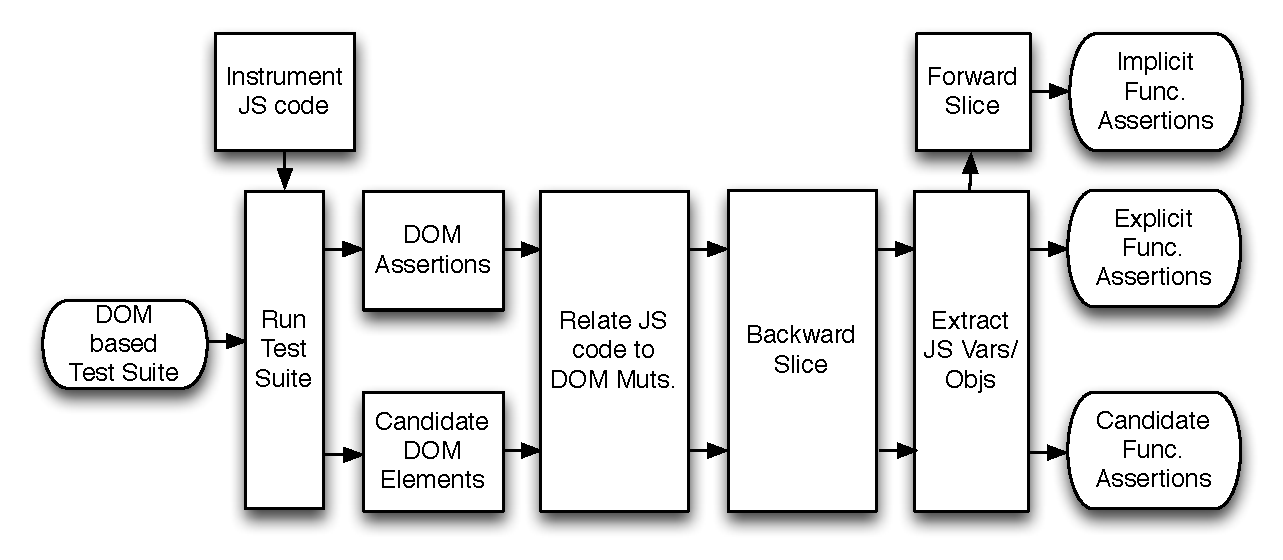
\includegraphics[width=.7\hsize]{fig/approachDiagram}
  \mycaption{Overview of our assertion generation approach.}
  \vspace{-0.1in} 
  \label{Fig:approachDiagram}
  \vspace{-0.1in} 
\end{figure*}
An overview of our \javascript function-level assertion generation technique is depicted in \figref{approachDiagram}.
At high level, our approach generates function level assertions for the \javascript code by utilizing human written DOM-based tests and assertions. Our code level assertions fall in the following three categories: (1) explicit assertions, which are directly inferred from analyzing the manually written DOM-based assertions, (2) implicit assertions, which are indirectly affected by the human written DOM-based assertions, and (3) candidate assertions, which are not considered in the written DOM-based assertions, yet are potentially useful to be checked by the function level test suite. We describe our approach below. The numbers below in parentheses correspond to those in the boxes of \figref{approachDiagram}.

In the first part of our approach we (1) instrument the \javascript code and execute the instrumented application by running the existing DOM-based test suite. In this step we gather a detailed execution trace of the application. We then extract (2) DOM-based assertions, and (3) candidate DOM element properties, which are useful DOM properties that can potentially be utilized for the purpose of assertion generation. We (4) identify the initial point of connection between the \javascript code and checked DOM element. We collect lines of code responsible for updating the corresponding DOM element. After determining DOM mutating statements, we (5) calculate the backward slice of these statements to find the entire code blocks that update the checked DOM element. We (6) extract \javascript entities including variables and objects associated with each of the obtained statements. Accessible entities form our explicit function level assertions (7). We further (8) perform a forward slice on the extracted \javascript entities to identify statements, that are implicitly affected by such entities. The accessible \javascript variables/objects associated with collected statements form our implicit function level assertions (9). In addition to explicit and implicit assertions, we also generate candidate assertions (10). Candidate assertions are involved with updating potentially useful DOM element properties, which are not checked in the existing DOM-based assertions. To obtain candidate function level assertions, we perform step (4), (5), and (6) on the inferred candidate DOM element properties (3).

Our overall unit-level assertion generation is presented in \algref{algorithm}. In the following sections we describe our technique for extracting DOM related information from the execution (\secref{extractDomRelatedInfo}), relating
DOM mutations to the \javascript code (\secref{domToCode}), and generating unit test assertions (\secref{unitLevelAssertion}).   
\subsection{Extracting DOM-Related Characteristics} \label{Sec:extractDomRelatedInfo}
The DOM connects a test case to the web application's code. Therefore, we first need to analyze the DOM-based test suite and extract the following pieces of information: (1) DOM-related operations of the existing test suite that may have tight connection with the \javascript code, and (2) frequently accessed DOM properties, which potentially are potentially influential in improving the fault finding capability of the test suite, but left unchecked in the manually-written test suite.
\headbf{DOM-Related Operations}
Any written test case needs to check the correctness of the application's behaviour. In a DOM-based test case the expected behaviour is checked through DOM-based assertions.
DOM-based assertion is defined as $<DOMProp,ExpVal>$, where $DOMProp$ is a DOM element feature (e.g. attribute, and/or textual value), and $ExpVal$ is the correct value expected by the assertion. Through the rest of the paper, we call DOM element feature as DOM property. 
DOM-based assertions play a significant role in our approach as they can guide us towards important portions of the underlying \javascript code that need to be checked in unit-level assertions.

For each DOM-based assertion we find \emph{Intra DOM assertion correlation} within the test suite.
\begin{mydef}[Intra DOM Assertion Correlation]
An intra DOM asseetion correlation is defined as a three tuple of $<DOMProp, AccDOM, AccDOMDep>$, where $DOMProp$ is the accessed DOM property within the assertion, $AccDOM$ is the accessed DOM elements in the test case pertaining to the assertion, and $AccDOMDep$ is the DOM dependencies of the assertion in the test case.
\end{mydef}
\textsc{GetDomAcc} in line 10 of \algref{algorithm} retrieves DOM dependencies of the assertion in the test case.
%, we instrument the test case by wrapping around method calls that accesses DOM elements.
Going back to our example in \figref{example}(b), tracking the assertion in line 11 shows that it has a DOM dependency to a \code{div} element with class \code{shopContainer}, which is accessed in line 10.

We further need to link the inferred Intra DOM assertion correlation with the application's code.
We call the correlation between the DOM-based assertion and the \javascript code of the application as \emph{inter DOM assertion correlation}.
\begin{mydef}[Inter DOM Assertion Correlation]
An inter DOM assertion correlation is defined as\\
$<AccDOMDep, InitCode>$, where $InitCode$ is the initial point of contact in the application's code segment, that is responsible for mutating $AccDOMDep$ the previously extracted DOM elements from the test suite.
\end{mydef}
To infer this type of correlation we track DOM's evolution of the $AccDOMDep$ (\textsc{GetDomMuts} in line 13 of the algorithm) as well as invoked event handlers as the test case runs. 
We consider additions and removals of child nodes, changes to attributes, and updates to child text nodes as DOM mutations. For instance, running the sample test case in \figref{example}(b) results in mutating (1) the textual value of \code{div} element with class \code{shopContainer}.
%We call the correlation between the DOM-based assertion and the \javascript code of the application as \emph{inter DOM assertion correlation}. This correlation is defined as $<AccDOMDep, InitCode>$, where $InitCode$ is the initial point of contact in the application's code segment, that is responsible for mutating the previously extracted DOM elements from the test suite ($AccDOMDep$).  
%We make use of \code{document.onload} event to log the initial DOM state. 
%An observer module is then used to monitor mutations on the DOM during the test case execution. 
%In addition to DOM changes, we also keep track of \javascript events as well as invoked event handlers. This information is later used to find the initial point of contact between a DOM mutation and the executed code segments.
%For instance, running the sample test case in \figref{example}(b) results in mutating (1) the textual value of \code{div} element with class \code{shopContainer}, and (2) the \code{class} attribute of DOM element with ID \code{couponButt}.
\headbf{Frequently Accessed DOM Properties}
In addition to DOM-based assertions, we further consider DOM element properties, that are frequently accessed within the application as the test case runs (lines 1 to 7 of \algref{algorithm}). 
\textsc{Acc} in line 6 of the algorithm computes the access frequency of a DOM property, $freqAccdDOM$ in line 7 contains the inferred candidate DOM properties, and \textsc{GetDomMuts} in line 19 records DOM mutations occur
on candidate DOM properties.
The intuition is that frequent use of a given DOM property can point to the extent of application's behaviour dependency on the DOM property. Thus, if changes happen to that property through the \javascript code, it is important to assert the correctness of such mutations. We define the access frequency of a DOM element property as the number of times that the element's property has been read during the execution of a test case. DOM properties include attributes as well as textual value of the elements.
In order to record DOM property accesses within the application, we rewrite native function calls used by programmers to access DOM element such as \code{getElementById}, \code{getElementsByClassName}, and/or \code{getElementsByTagName}. The returned object from these functions is later used to access attributes or textual values of the element. Thus, we apply a forward slice on the returned object to find instances of element's property access in the code.
For example in function \code{addToCart} of \figref{example}(a), DOM element with ID \code{couponButt} is assigned to \code{coupElem} variable. The assigned variable is later used to access the \code{class} attribute as well as the \code{value}
of the DOM element in lines 23, 25, and 26.

Let $Acc(prop_{el})$ be the access frequency computed for property $prop$ of DOM element $el$, then:
 
$Acc(prop_{el})=\frac{Read(prop_{el})}{\sum _{e=1}^{n} Read(domElem_e)}$, where $Read(domElem_{e})$ is the number of times that DOM element $domElem$ is read, given that the total number of DOM elements during the execution of a test case is $n$.
Note that reading a DOM element refers to accessing the element to read the corresponding property. In \figref{example}(a), the \code{class} attribute of DOM element \code{couponButt} is read in lines 23 and 34, and thus the access frequency
computed for the \code{class} attribute of the element is equal to $\frac{2}{3}$.

We choose element's property with access frequencies above a threshold $\alpha$ as potential candidates, which are later used for the purpose of unit-level assertion generation. We automatically compute this threshold for each test case as: 

$\alpha=\frac{1}{ReadProperties(T)}$, where $ReadProperties(T)$ is the total number of properties which have been read during the execution of test suite $T$.

Going back to our running example and the sample DOM-based test case in \figref{example}, \code{class} attribute of the \code{couponButt} is selected as a potential candidate since its access frequency ($\frac{2}{3}$) is greater than the computed threshold, which is equal to $\frac{1}{2}$ in this example.        
%application instrumentaion native event wrapping    

\subsection{Relating DOM Changes to the Code} \label{Sec:domToCode}
%\IncMargin{0em}
\begin{algorithm}[t]
{\scriptsize
\SetKwInOut{Input}{input}\SetKwInOut{Output}{output}
\Input{Test suite $T$; The set of test cases $tc_i \in T$}
\Output{The ordered set of oracles $oracles$}
\BlankLine

\Begin {
\nl \For{$tc_i \in T$}{
\nl  $trace \leftarrow textsc{Exec}(tc_i)$\\
\nl  $domAccss \leftarrow \textsc{GetDOMAcc}(trace)$\\   	
\nl  $freqAccdDOM\leftarrow \emptyset$\\
\nl  \For{$dom \in domAccss $}{
\nl   \If{$\textsc{DOMUsgFreq}(dom) \geq \frac{1}{NoOfDOMElems} $}{
\nl    $freqAccdDOM \leftarrow dom \cup freqAccdDOM$\\       
      }
     }
\nl  \For{$asstn \in assertions_{tc_i}$}{
\nl   $asserDOMAcc \leftarrow \textsc{GetDOMAcc}(asstn)$\\
\nl   $asserDOMMuts \leftarrow \textsc{GetDOMMuts}(asserDOMAcc)$\\
\nl   \For{$domMut \in asserDOMMuts$}{
\nl    $bwSts \leftarrow \textsc{GetBWSlice}(domMut, trace)$\\
\nl    $asstnRel \leftarrow \textsc{GetWrVars}(bwSts)$\\
\nl    $potAsstnRel \leftarrow \textsc{GetFWSlice}(asstnRel, trace)$\\
      }
     }
\nl  $nonAsserDOMMuts \leftarrow \textsc{GetDOMMuts}(freqAccdDOM)$\\
\nl  \For{$domMut \in nonAsserDOMMuts$}{
\nl   $bwSts \leftarrow \textsc{GetBWSlice}(domMut, trace)$\\
\nl   $nonAsstnRel \leftarrow \textsc{GetWrVars}(bwSts)$\\
     }
\nl  $asstnRelOrcls[func]_{f=1}^{n} \leftarrow \textsc{GetValue}(\textsc{Accessibles}([func]_{f=1}^{n}, asstnRel))$\\
\nl  $candidOrcls[func]_{f=1}^{n} \leftarrow \textsc{Accessibles}([func]_{f=1}^{n}, [potAsstnRel \cup nonAsstnRel])$\\
\nl  $oracles[func]_{f=1}^{n}.\textsc{Add}(asstnRelOrcls \cup candidOrcls)$\\
   }
\nl $\textsc{Rank}(oracles[func]_{f=1}^{n})$\\
\nl return $(oracles[func]_{f=1}^{n})$
}
\caption{Oracle Generation} 
\label{Alg:algorithm}
}
\end{algorithm}
%\DecMargin{lem}
\begin{figure}[!t]
  \centering
  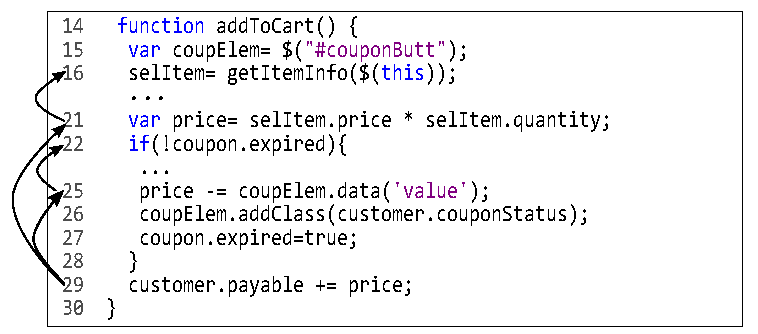
\includegraphics[width=1\hsize]{fig/intraCodeDep}
  \vspace{-0.3in} 
  \mycaption{Intra (data and control) code dependency through backward slicing.}
  \label{Fig:intraCodeDep}
  \vspace{-0.2in} 
\end{figure}
To determine the initial point of contact between DOM and the underlying application's code, we first cross reference the DOM element as well as the property we are interested in with a set of DOM mutations obtained from the execution trace. The desired DOM element and its property are inferred from either the intra DOM assertion dependency or the candidate DOM properties as described in \secref{extractDomRelatedInfo}. Recall that our execution trace contains information about triggered events, event handlers, and DOM mutations caused by the events. Therefore, we can identify relevant events and invoked functions corresponding to a given DOM mutation.
For example, the collected execution trace in \figref{assertionToCode} contains information about the mutations of a \code{div} element with class \code{shopContainer}, which pertains to the DOM-based assertion.

To figure out where the mutation originated in our execution trace, we keep record of DOM accesses within the invoked functions. For each DOM access, we track \javascript lines of code that are responsible for updating the corresponding DOM element. Going back to our example in \figref{assertionToCode}, given that the textual property of the \code{div} element is extracted from the intra DOM assertion dependency, we identify line 30 in function \code{viewCart} as the initial point of contact responsible for changing the \code{text} of DOM element.

After inferring DOM mutant statements, we identify the control and data \emph{intra code dependency} within the application's code.
%gather the entire set of \javascript statements responsible for mutating a given DOM element.
\begin{mydef}[Intra Code Dependency]
\label{def:intraCodeDep} 
 
An intra code dependency is defined as $<criterion, codeSts>$, where $criterion$ is a variable at the initial point of contact, and $codeSts$ is the set of control and data dependent statements that are either affected by the $ctiterion$ or have some effect on the $criterion$. 
\end{mydef}

To find the intra code dependency, we perform backward as well as forward slicing by using $criterion$ as the slicing criterion.
\textsc{GetBWSlice} in lines  15 and 21 of \algref{algorithm} computes a backward slice with respect to assertion related DOM mutations, and candidate DOM property mutations respectively.
We use dynamic slicing to capture run-time dependencies.
Note that instrumenting the entire application's code to perform dynamic slicing incurs high performance overheads. To avoid high overheads, we first intercept the code sent from the server to the client, and then statically instrument only those statements that may affect a given DOM element.
To extract the subset of the code statements, we first find the \javascript closure scope which contains the definition of the variable in the initial slicing criteria. Then all references to the variable within the closure scope are found. Therefore, we can identify all locations in the code where the variable is updated, read, or a new alias is created. For each variable update/read related to the variable of the slicing criteria, we track the data dependencies for such an operation. The aforementioned steps are performed iteratively for each dependencies to collect the subset of code statements, which are instrumented for a given initial slicing criteria.
The instrumented code keeps track of all updates and accesses to all relevant data and control dependencies.   
Once the test case runs, we collect traces from the instrumented code. This trace is used to dynamically extract backward slicing as well as forward slicing statements. Note that in addition to backwards slicing which is later used to generate explicit assertions, we also use forward slicing to generate our implicit assertions (\secref{implicitAssertions}).  

The backward slicing technique starts by extracting instances of the initial slicing criteria from the trace. For each \textit{read} operations, the trace is traversed backwards to find the nearest related \textit{write} operation. Once found, the \textit{write} operation is added to the slice under construction. This process is repeated for all the data dependencies related to that write operation. A similar approach is taken for including control dependencies in the slice. 
Our slicing technique supports inter-procedural slicing. For example, if a variable is assigned by the return value of a called function, the slicer recursively tracks the function and performs a backward slice on the statement returned by the called function.
%We track the following types of function calls during the slicing process: (1) Regular function calls e.g. \code{func()}, (2) Method calls e.g. \code{obj.func()}, (3) Constructors e.g. \code{new func()}, (4) Function handlers e.g. \code{element.click(func)}, and (5) Anonymous functions, which are assigned to a variable or an object property.
  
To address aliasing when computing the slice of a variable that has been set by a non-primitive value, we need to consider possible aliases that may refer to the same object. Specifically in \javascript \textit{dot notation} and \textit{bracket notation} are frequently used to modify objects at run time. Since static analysis techniques for \javascript often ignore this issue \cite{Feldthaus:icse13}, we use dynamic slicing. If a reference to an object of interest is saved to a second object's property, e.g. through the use of the \textit{dot notation}, the object of interest may also be altered via aliases of the second object. For example, after executing statement \code{a.b.c = objOfInterest;}, updates to \code{objOfInterest} may be possible through \code{a}, \code{a.b}, or \code{a.b.c}. To deal with such scenarios, our slicing technique searches through the collected trace and adds the forward slice for each detected alias to the current slice for our variable of interest (e.g. \code{objOfInterest}). 

Given \code{customer.payable} as the initial slicing criteria in our example, \figref{intraCodeDep} shows the relevant backward slice statements (lines 22, 18, 15, 14, and 9), where \code{customer.payable},  variable \code{price}, as well as properties of the object \code{selItem} are assigned, and the value of \code{coupon.expired} is checked in the conditional statement.
By the end of backward slicing step, we have all the relevant statements corresponding to a given DOM element. These are later used to derive test assertions.    
\subsection{Generating Unit-Level Assertions} \label{Sec:unitLevelAssertion}
Our approach targets postcondition assertions which are used to examine the expected behaviour of a given function after it is executed in a unit test case.
Through analyzing a given DOM-based test case, we generate unit-level assertions in the following three categories: (1) assertions, which are directly related to a given DOM-based assertion, (2) assertions, which are indirectly affected by a given DOM-based assertion, and (3) assertions that have direct impact on important DOM elements which are not checked by the existing DOM-based assertions. Each assertion is coupled with the expected value obtained from the execution trace of the application. The first type of assertion (type 1), which we call explicit assertion, can potentially be used in unit testing of the current version of the application. Type 2 and type 3, which we call implicit assertions and candidate assertions respectively, can be used for the purpose of regression testing.
\subsubsection{Explicit Assertions} \label{Sec:explicitAssertions}
After collecting all the statements, that are relevant to a given DOM-based assertion, we extract accessible entities from these statements (\textsc{Accessibles} in line 23 of the algorithm).
Types of accessible entities include (1) the function's returned value, (2) the used global variables in that function, (3) the object's property where the object is accessible in the outer scope of the function, and/or (4) the accessed DOM element in that function. Dynamic backward slice of a DOM-based assertion helps to (1) track all statements that contribute to the checked result and as such identify those entities that might have influenced the checked property value of the DOM element, and (2) eliminate unrelated entities that are not involved in the computation that leads to the update performed on the checked DOM element.

Since our dynamic slice is extracted from the program run, we can track all concrete values associated with accessible entities.
During the run of a test case, there might be different instances where a given statement is executed. Different execution instances can lead to different behaviour. Since we are using dynamic slicing, an instance that leads to the required behaviour, which is checked through the DOM-based assertion, is on the backward slice. Given that the manually-written expected value, that is checked against the DOM's property is valid, the concrete values of related entities in the backward slice are potentially correct. Therefore, concrete value of an entity in the backward slice can be used as the expected value of the entity in unit-level assertions to test the current version of the application (discussed in \secref{discussion}).
$explicitAsstn$ in line 23 of \algref{algorithm} contains the inferred explicit assertions.

In our running example (\figref{intraCodeDep}), explicit assertions check the correctness of \code{customer.payable}, \code{coupon.expired}, as well as \code{price} and \code{quantity} properties which belong to \code{selItem} object.
Assuming that the original price of the item is 100, the number of selected item is 1, and the calculated discount according to the \code{value} attribute of a DOM element with ID \code{couponButt} is 30, then the expected values included in the assertions for each of the entities are 70, boolean value \code{true}, 100, and 1, respectively. \figref{unitTest} shows a unit test case for \code{addToCart} function with the generated assertions in \qunit framework. %\karthik{What's a \qunit test?} 
Lines 7 to 9 in the figure corresponds to the explicit assertions.
\begin{figure}
  \centering
  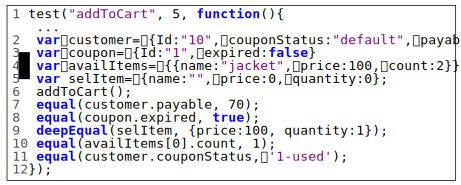
\includegraphics[width=1\hsize]{fig/unitTest}
   \vspace{-0.3in} 
  \mycaption{Generated \qunit test case and assertions.}
  \label{Fig:unitTest}
  \vspace{-0.28in} 
\end{figure}  
%We compare the value of the entity immediately after the relevant statement is executed in the backward slice with the entity's value before the function exits. If value of the entity remains the same, we use it towards the expected value in the unit-level assertion.  
%However, if the entity pertaining to a DOM change is reassigned in the code after the DOM gets updated and before the function exits, then the concrete value of the entity can be used for the purpose of regression testing unless the tester provides the proper expected value.
\subsubsection{Implicit Assertions} \label{Sec:implicitAssertions}
To this end we gather all the statements that explicitly affect the computations relevant to a given DOM-based assertion. While assertions inferred from such statements are inherently important, we further need to consider entities that are implicitly influenced by the checked DOM element in the manually-written test suite. For this purpose we apply a dynamic forward slice on the statements collected from a backward slice of a DOM-based assertion. A forward slice with respect to a statement $st$,
indicates how subsequently an operand at $st$ is being used. This can help the tester to ensure that $st$ properly establishes the expected outcome of the computations assumed by the later statements. 
Given the importance of statements involved in code-level computations of a DOM-based assertion, using forward slice is useful to check that there are no unforeseen effects on the application's behavior by a modification to such statements. 

Dynamic forward slice is performed on the subset of code statements which is previously instrumented as explained in \secref{domToCode}. The process of forwards slicing is similar to the backwards slicing technique as discussed earlier (\secref{domToCode}). The only difference is that it is performed in a forward direction. The slicing criterion of the forward slice module is either a variable, object's property, or an accessed DOM property extracted from the statements in a backward slice. The accessible entities, which have been set within the collected forward slice statements establish our implicit assertions.   
\subsubsection{Candidate Assertions} \label{Sec:candidateAssertions}
In addition to explicit and implicit assertions, we also verify the correctness of code-level entities pertaining to DOM updates, which are essentially important but not checked in the existing DOM-based test cases. We derive such unit-level assertions, namely candidate assertions, from the candidate DOM element properties previously obtained from the test case execution (box 3 in \figref{approachDiagram}). As the test case runs, we monitor DOM's evolution and match the list of mutated DOM elements and their properties with property updates of the candidate DOM elements. Once a match is found, we infer backwards slice statements pertaining to the mutation of DOM element's property (\textsc{GetBWSlice} in line 18 of the algorithm). Therefore, in this case the slicing criteria which is given as input to the backwards slicing module is an update to the property of the candidate DOM element.
After gathering the related \javascript statements within the application, we extract accessible entities of these statements (\textsc{Accessibles} in line 22) which form our candidate assertions. $candidateAsstn$ in line 22 contains our candidate assertions. 

Recall from the example (\figref{example}), one such potential DOM property which we record as part of \secref{extractDomRelatedInfo}, is \code{class} attribute associated with DOM element with ID \code{couponButt}. Monitoring DOM changes reveal that line 26, where the \code{class} attribute of the element is set, is the initial point of contact between DOM mutation and the \javascript code. Given line 26 as the slicing criteria, \code{customer.couponStatus} (line 24) is marked as the candidate assertion.
          
%mutation of customer.couponStatus = coupon.Id + '-' + 'used' to customer.couponStatus = coupon.Id + 'used';'
\subsection{Tool Implementation: Atrina} \label{Sec:tool}

We have implemented our \javascript unit test assertion generation in an automated tool called \atrina. The tool is written in Java, and is publicly available for download \cite{atrina-dl}.
We use a proxy server to intercept HTTP responses which contain \javascript code. The \javascript Mutation Summary library \cite{mutationSummary} is used to track DOM changes during the execution of the test suite. Trace information is collected by the proxy once received from the browser. To instrument Selenium test cases, we convert them into an abstract syntax tree (AST) by employing Eclipse Java development tools (JDT). Once the transformation is done, we run the Java code of the changed AST on the application under test.   


\section{Empirical Evaluation} \label{Sec:evaluation}

To quantitatively assess the efficacy of our test generation approach, we have conducted an empirical study, in which we address the following research questions:

\begin{table*}
\centering
%\vspace{5pt}
        \caption{Characteristics of the experimental objects.}
{\scriptsize
    \begin{center}
       
      %  \subtable[Experimental subjects and the corresponding exploration data]
            {
           \begin{tabular}{c|l|c|c|c|l} \hline
\thead{App ID} &\thead{Name} &\thead{JS LOC} & \thead{\# Functions} &\thead{CC} &\thead{Resource}  \\  \hline \hline

1  & SameGame & 206 & 9 & 37 & \url{http://crawljax.com/same-game}   \\ \hline
           
2 & Tunnel & 334 & 32  & 39 & \url{http://arcade.christianmontoya.com/tunnel} \\ \hline

3 & GhostBusters & 277 & 27 & 52 & \url{http://10k.aneventapart.com/2/Uploads/657}  \\ \hline

4 & Symbol & 204 &  20 & 32  & \url{http://10k.aneventapart.com/2/Uploads/652}\\ \hline

5 & TuduList & 2767 &  229 & 28  & \url{http://tudu.ess.ch/tudu}\\ \hline

6 & SimpleCart (library) & 1702 & 23  &  168 & \url{http://simplecartjs.org}\\ \hline

7 & \jquery (library)& 8371  &  45 & 37  & \url{https://github.com/jquery/jquery}\\ \hline

8 & WymEditor & 3035  &  188 & 50  & \url{https://github.com/wymeditor}\\ \hline

\hline\end{tabular}\centering
            }
\label{Table:objectsChar-table}
\end{center}
}  
\vspace{-0.1in} 
\end{table*}

\begin{description}[noitemsep]
%\item [RQ1] How effective is our \emph{function coverage maximization} technique?
\item [RQ1] How effective is \tool in generating test cases with high coverage? 
\item [RQ2] How capable is \tool of generating test oracles that detect regression faults?
\item [RQ3] How does \tool compare to existing automated \javascript testing frameworks?
\end{description} 

%in which we compare \tool with an existing \javascript testing tool \artemis

\tool and all our experimental data produced are available for download \cite{jseft-dl}.



\subsection{Objects}
Our study includes thirteen \javascript-based applications in total. 
\tabref{objectsChar-table} presents each application's ID, name, lines of custom \javascript code (LOC, excluding \javascript libraries) and resource.
The first five are web-based games. AjaxTabs is a \jquery plugin for creating tabs. NarrowDesign and JointLondon are websites. FractalViewer is a fractal tree zoom application. SimpleCart is a  shopping cart library, WymEditor is a web-based HTML editor, Tudu\-List is a web-based task management application, and Tiny\-MCE is a \javascript based WYSIWYG editor control. The applications range from 206 to 27K lines of \javascript code.
%which has been used in other studies  \cite{artzi:icse11}. 

The experimental objects are open-source and cover different application types. All the applications are interactive in nature and extensively use \javascript on the client-side. %Since we require automated access and modification of the source code (\ie for instrumentation), we were not able to use applications such as FaceBook, where automated access is forbidden. %Moreover, since \tool does not support server-side testing, applications which their computations are mostly performed on the server side do not benefit from our approach.    


\subsection{Setup} \label{Sec:setup}
To address our research questions, we provide the URL of each  experimental object to \tool.
Test cases are then automatically generated by \tool.
%It is believed that \cite{humble:2010} testers dedicate no more than 10 minutes to test execution. Therefore, 
We give \tool 10 minutes in total for each application. 
5 minutes of the total time is designated for the dynamic exploration step.
%We outline the setup and methodology used in our empirical study to address our research questions.

%\subsubsection{Function Coverage Maximization (RQ1)}
%To measure the effectiveness of the function coverage maximization technique, we provide the URL of each experimental object to the first component of \tool as depicted in \figref{approach-view}. We compare our state/event selection strategy with a random exploration method, in which the next state is chosen uniformly at random for the expansion. 
%We limit the dynamic exploration time to five minutes \cite{humble:2010} for each technique and report the average results over five runs. We generate event sequences from the two state-flow graphs obtained from each method. 
%
%\jscover \cite{jscover}, an open-source tool for measuring \javascript code coverage, is used to measure the statement coverage. We collect the traces of the executed statements after each event is triggered. 
%Finally, we compare the statement coverage achieved by running the generated event sequences separately.
\headbf{Test Case Generation (RQ1)} \label{test-gen-setup}
To measure client-side code coverage, we use \jscover \cite{jscover}, an open-source tool for measuring \javascript code coverage. We report the average results over five runs.
In addition,  we assess each step in our approach separately as follows: 
(1) compare the statement coverage achieved by our function coverage maximization with a method that chooses the next state/event for the expansion uniformly at random, 
(2) assess the efficacy of our function state abstraction method (\algref{stateAbstractionAlgo}), and 
(3) evaluate the effectiveness of applying mutation techniques (\algref{oracleGenAlgo}) to reduce the number of assertions generated.
% we provide the URL of each experimental object to the first component of \tool as depicted in \figref{approach-view}. We compare our state/event selection strategy with a random exploration method, in which the next state is chosen uniformly at random for the expansion. 
%We generate event sequences from the two state-flow graphs obtained from each method. 

%We collect the traces of the executed statements after each event is triggered. 
%Finally, we compare the statement coverage achieved by running the generated event sequences separately. 

%Of course, no unit test generation technique can test functions that are not directly accessible (\eg nested functions, anonymous functions).
%Therefore, in addition to measuring the statement coverage of the generated test suite, we define a unit testability metric, which measures the testability degree of individual functions of an application. We call a function $f$ \emph{testable} if it is possible to call $f$ directly from a test case --- regardless of whether the test case is written manually or generated automatically. The testability metric of a given web application $A$ is calculated as follows: 
%
%\begin{equation}
%testability(A)=\frac{\sum _{i\in A(f_i)}^{n} {testable(f_i)}}{n},
%\label{testabilityFormula}
%\end{equation}
%\noindent
%where $n$ is the total number of functions, and $testable$ decides whether a function ($f_i$) is testable according to the definition. We then measure the percentage of functions that \tool can generate test cases for in $A$ as:   
%
%\begin{equation}
%testGenRate(A)=\frac{\sum _{i\in A(f_i)}^{n} {tested(f_i)}}{\sum _{i\in A(f_i)}^{n} {testable(f_i)}},
%\label{pythiaTestabilityFormula}
%\end{equation}
%\noindent
%where the numerator is the total number of functions that are directly tested by \tool and the denominator is the total number of testable functions in $A$.

\headbf{Test Oracles (RQ2)} \label{test-oracle-setup}
%To generate test oracles at function-level, we configure \tool to inject 50 \javascript code-level faults in each application.
%To produce DOM event-level oracles, we configure the DOM mutation module of \tool to inject 20 DOM-level faults per application. \ali{why 50? why 20? why these numbers? why are they not the same? Motivate! Do we need to include this information?} %We then run \tool on each web application to obtain the test cases with oracles.
%
To evaluate the fault finding capability of \tool (RQ2), we simulate web application faults by automatically seeding each application with 50 random faults. %according to the following fault category: 
%\begin{enumerate}[noitemsep, nolistsep]
%\item Changing conditional statements by modifying the upper/lower bounds of loop statements, 
%changing the condition itself, as well as swapping consecutive conditional statements;
%\item Modifying the values of global/local variables, and removing or changing their names, as well as modifying arithmetic operations;
%\item Changing function parameters or function call arguments by swapping, removing,
%and renaming parameters/arguments. Changing the sequence of function
%calls within a given function if applicable;
%\item Modifying DOM related properties.
%\end{enumerate}
%The first three categories target \javascript code while the last one targets both \javascript and HTML code-levels. 
We automatically pick a random program point and seed a fault at that point according to our fault category.
While mutations used for oracle generation have been selectively generated (as discussed in \secref{oracleGen}), 
mutations used for the purpose of evaluation are randomly generated from the entire application. Note that if the mutation used for the purpose of evaluation and the mutation used for generating oracles happen to be the same, we remove the mutant from the evaluation set. 
%in the \javascript code as well as the HTML code of each application. 
%Note that we decided to manually perform fault seeding instead of using \mutandis, which automates \javascript mutation testing. The main reason is to mitigate bias since \mutandis is used by \tool to generate mutants automatically during the test oracle generation phase. 
%One challenge with generating assertions is their stability, \ie the assertions may fail on the original version of the program. To filter unstable assertions, we run the test suite on the original program and discard any assertions that fail.
%
Next we run the whole generated test suite (including both function-level and event-based test cases) on the faulty version of the application. The fault is considered detected if an assertion generated by \tool fails and our manual examination confirms that the failed assertion is detecting the seeded fault.
%\ali{how do we know we have detected the right fault?}
We measure the precision and recall as follows:

\begin{description}[noitemsep, nolistsep]
\item[Precision] is the rate of injected faults found by the tool that are actual faults: $\frac{\mathit{TP}}{\mathit{TP} + \mathit{FP}}$
\item[Recall] is the rate of actual injected faults that the tool finds: $\frac{\mathit{TP}}{\mathit{TP} + \mathit{FN}}$ 
\end{description}
where $\textit{TP}$ (true positives), $\textit{FP}$ (false positives), and $\textit{FN}$ (false negatives) respectively represent the number of faults that are correctly detected, falsely reported, and missed.

\headbf{Comparison (RQ3)} \label{comparison-setup}
To assess how \tool performs with respect to existing \javascript test automation tools, we compare its coverage and fault finding capability to that of \artemis \cite{artzi:icse11}.  
Similar to \tool, we give \artemis 10 minutes in total for each application; we observed no improvements in the results obtained from running \artemis for longer periods of time. 
We run \artemis from the command line by setting the iteration option to 100 and enabling the coverage priority strategy, as described in \cite{artzi:icse11}. %\karthik{Earlier you said 5 minutes}. 
Similarly, JSCover is used to measure the coverage of \artemis (over 5 runs).
We use the output provided by \artemis to determine if the seeded mutations are detected by the tool, by following the same procedure as described above for \tool. 
%We measure the coverage using the HTML output of \artemis, which shows the covered \javascript code. %As mentioned before, we measure the coverage of \tool using \blanket.


\subsection{Results} \label{Sec:results}

%\begin{table}
%\vspace{5pt}
        \caption{Code coverage achieved for test cases generated by \tool and \artemis.}
{\scriptsize
    \begin{center}
       
      %  \subtable[Experimental subjects and the corresponding exploration data]
            {
           \begin{tabular}{c|c|c} \hline
\thead{App ID} &\theadturn{\tool (\%)} &\theadturn{\artemis  (\%)}  \\  \hline \hline

1  & 99 &  92 \\ \hline
           
2 & 78 &  49 \\ \hline

3 & 90 & 35 \\ \hline

4 & 75 &  65 \\ \hline

5 & 49 &  15 \\ \hline

6 & 78 &  66 \\ \hline

7 & 63 &  0 %30
 \\ \hline

8 & 56 & 0 % 42
  \\ \hline

9 & 82 &  63 \\ \hline

10 & 71 & 67  \\ \hline

11 & 56 &  46 \\ \hline

AVG& 72.5 & 45.3 \\ \hline


\hline\end{tabular}\centering
            }
\label{Table:covg-table}
\end{center}
}
\end{table} 


%\headbf{Function coverage maximization (RQ1)} \tabref{efficiency-abs-mut-table} presents the statement coverage achieved by using our function coverage maximization technique and the random strategy. Our results show on average 9\% improvement in statement coverage, across all the applications. We observed that our technique achieves the highest improvement when there are dynamically generated clickables in the application.
%
%For example, for Tunnel (ID 2) and Fractal Viewer (ID 9), we observed no improvement in the statement coverage as these two applications have no dynamically generated or bound to event-listeners clickables. Instead, their few clickables are all placed in the HTML code of the application with a fixed event-handler per clikcable. Thus,  our approach achieves the same coverage as the random strategy for such applications.
%
%For SameGame (ID 1) the number of executed functions remains the same, for both approaches. However, in the limited five minute period of time, as a result of dynamically detecting valid clickable elements, \tool is able to examine different paths of the applications, while the random exploration technique fails to do so as it blindly clicks on any candidate element on the DOM tree.
%
%Finally, GhostBusters (ID 3) benefits the most from our dynamic exploration technique. This application contains a large number of dynamically created clickable DOM elements that appear and then disappear within a few seconds. We observed two anonymous functions, attached to clickable elements, that are missed by the random exploration technique in this application. Our technique is not only able to quickly spot such on the fly generated clickables, but it is also able to click on the ones that result in the execution of uncovered functions. 
%These two functions are attached to clickable elements that are not executed using random strategy. 

\begin{table}
\center
%\vspace{5pt}
        \caption{Results showing the effects of our \textbf{function coverage maximization}, \textbf{function state reduction}, and \textbf{mutation-based oracle generation} algorithms.}
        \label{Table:efficiency-abs-mut-table}
{\scriptsize
       
      %  \subtable[Experimental subjects and the corresponding exploration data]
            {
           \begin{tabular}{c|r|r||r|r|r||r|r} \hline
&\multicolumn{2}{c||}{\thead{St. Coverage}} & \multicolumn{3}{c||}{\thead{State Reduction}} & \multicolumn{2}{c}{\thead{Oracles}}\\
\cline{2-8}

\theadturn{App ID} &

\theadturn{Fun. cov. maximize (\%)} & \theadturn{Random exploration (\%)} 
&\theadturn{\#Func.States w/o reduction} &\theadturn{\#Func.States with reduction}  &\theadturn{Func.State Reduction (\%)}
%&\multicolumn{2}{c}{\thead{Assertions}} \\ 
%\cline{5-6}&

&\theadturn{\#Assertions w/o mutation} &\theadturn{\#Assertions with mutation}  \\  \hline

\hline

1 & 99 & 80 & 447 & 42 & 91 & 5101 & 171\\ 

2 & 78 & 78 & 828 & 23 & 97 & 23212 & 91\\ 

3 & 90 & 66 & 422 & 22 & 95 & 3520 & 69 \\ 

4 & 75 & 75 & 43 & 18 & 58 & 1232 & 105\\ 

5 & 49 & 45 & 534 & 31 & 94 & 150 & 103\\ 

6 & 78 & 75 & 797 & 38 & 95 & 1648 & 149\\ 

7 & 63 & 58 & 1653 & 58 & 96 & 198202 & 365\\ 

8 & 56 & 50 & 32 & 23 & 28 & 78 & 67 \\ 

9 & 82 & 82 & 1509 & 51 & 97 & 65403 & 259 \\ 

10 & 71 & 69 & 71 & 22 & 69 & 6584 & 94 \\ 

11 & 56 & 54 & 1383 & 136 & 90 & 2530 & 334 \\ 

12 & 41 & 38 & 1530 & 64 & 96 & 3521 & 193 \\ 

13 & 51 & 47 & 1401 & 161 & 88 & 2481 & 361 \\ \hline

AVG& 68.4 & 62.8 & - & - & 84.1 & - & - \\  \hline
          
\hline\end{tabular}\centering
            }
}
\vspace{-0.18in}
\end{table}


%\begin{table}
%%\vspace{5pt}
%\centering
%        \caption{Results showing the effects of our \textbf{function coverage maximization}, \textbf{function state reduction}, and \textbf{mutation-based oracle generation} algorithms.}
%        \label{Table:efficiency-abs-mut-table}
%{\scriptsize
%       
%      %  \subtable[Experimental subjects and the corresponding exploration data]
%            {
%           \begin{tabular}{c|c|c||c||>{\centering}b{1.3cm}|c||>{\centering}b{1.3cm}|c||c|c} \hline
%&\multicolumn{2}{c||}{\thead{St. Coverage}} 
%& \multirow{3}{*}{\theadturn{\#Function states w/o state removal}} & 
%\multicolumn{2}{c||}{\thead{St. Reduction-Mutation}} & \multicolumn{2}{c||}{\thead{St. Mutation-Reduction}} & \multicolumn{2}{c}{\thead{Oracles}}\\
%\cline{2-3} \cline{5-10}
%
%\theadturn{App ID} &
%
%\theadturn{Fun. cov. maximize (\%)} & \theadturn{Random exploration (\%)} &&\theadturn{\#Func.States using Reduc-Mut }  &\theadturn{Func.State Reduction (\%)}
% &\theadturn{\#Func.States using Mut-Reduc }  &\theadturn{Func.State Reduction (\%)}
%%&\multicolumn{2}{c}{\thead{Assertions}} \\ 
%%\cline{5-6}&
%
%&\theadturn{\#Assertions w/o mutation} &\theadturn{\#Assertions with mutation}  \\
%&&&&&&&&& \\
%  \hline
%
%\hline
%
%1 & 99 & 80 & 447 & 33 & 93 & & & 5101 & 136\\ 
%
%2 & 78 & 78 & 828 & 21 & 97 & & & 23212 & 81\\ 
%
%3 & 90 & 66 & 422 & 14 & 96 & & & 3520 & 45 \\ 
%
%4 & 75 & 75 & 43 & 19 & 56 & & & 1232 & 109\\ 
%
%5 & 49 & 45 & 534 & 23 & 95 & & & 150 & 79\\ 
%
%6 & 78 & 75 & 797 & 30 & 96 & & & 1648 & 125\\ 
%
%7 & 63 & 58 & 1653 & 54 & 97 & & & 198202 & 342\\ 
%
%8 & 56 & 50 & 32 & 18 & 43 & & & 78 & 51 \\ 
%
%9 & 82 & 82 & 1509 & 49 & 97 & & & 65403 & 253 \\ 
%
%10 & 71 & 69 & 71 & 23 & 67 & & & 6584 & 96 \\ 
%
%11 & 56 & 54 & 1383 & 131 & 90 & & & 2530 & 318 \\ 
%
%12 & 41 & 38 & 1530 & 62 & 96 & & & 3521 & 184 \\ 
%
%13 & 51 & 47 & 1401 & 152 & 89 & & & 2481 & 335 \\ \hline
%
%AVG& 68.4 & 62.8 & - & - & 85.5 & & & - & - \\  \hline
%          
%\hline\end{tabular}\centering
%            }
%}
%\vspace{-0.18in}
%\end{table}

\begin{figure}[!t]
  \centering
  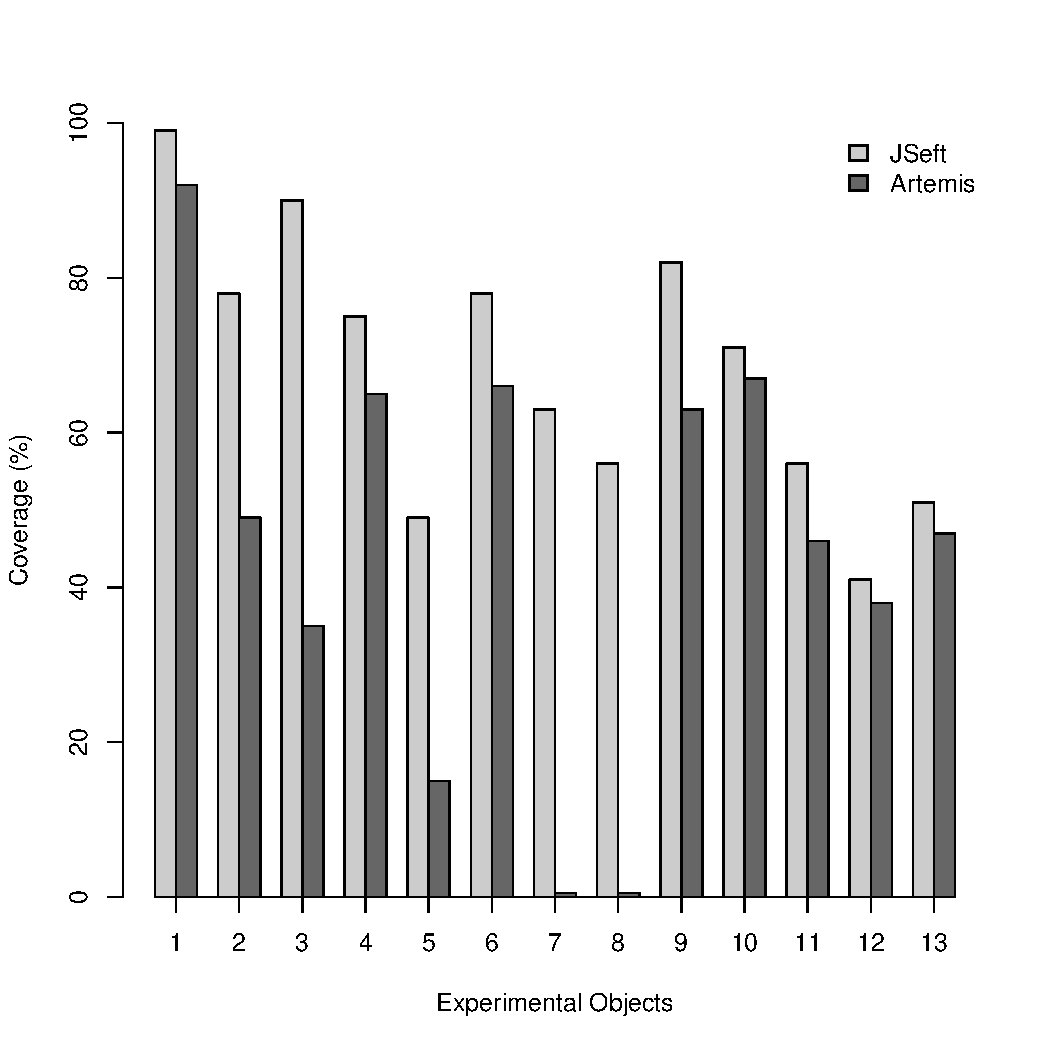
\includegraphics[width=1\hsize]{r-scripts/barplot_coverage}
  \vspace{-0.1in} 
  \mycaption{Statement coverage achieved.} 
  \vspace{-0.25in} 
  \label{Fig:coverage-graph}
\end{figure}


\headbf{Test Case Generation (RQ1)} 
\figref{coverage-graph} depicts the statement coverage achieved by \tool for each application. The results show that the test cases generated by \tool achieve a coverage of 68.4\% on average, ranging from 41\% (ID 12) up to 99\% (ID 1).
%\karthik{Do we need the text below ? We are better than random.}
We investigated why \tool has low coverage for some of the applications. For instance, we observed that in JointLondon (ID 7), the application contains \javascript functions that are browser/device specific, i.e., they are exclusively executed in Internet Explorer, or iDevices. As a result, we are unable to cover them using \tool. 
We also noticed that some applications required more time to achieve higher statement coverage (e.g., in NarrowDesign ID 8), or they have a large DOM state space (e.g., BunnyHunt ID 5) and hence \tool is only able to cover a portion of these applications in the limited time it had available.

\tabref{efficiency-abs-mut-table} columns under ``St. Coverage'' present \javascript statement coverage achieved by  our function coverage maximization algorithm versus a random strategy. The results show a 9\% improvement on average, for our algorithm, across all the applications. We observed that our technique achieves the highest improvement when there are many dynamically generated clickable DOM elements in the application, for example, GhostBusters (ID 3). 
%For instance, GhostBusters (ID 3) has 27\% more coverage since it contains a large number of dynamically created clickable DOM elements that appear and then disappear within a few seconds, which our technique can handle, but the random one may not. 
%We observed two anonymous functions, attached to clickable elements, that are missed by the random exploration technique in this application. Our technique is not only able to quickly spot such on the fly generated clickables, but it is also able to click on the ones that result in the execution of uncovered functions.

The columns under ``State Abstract'' in \tabref{efficiency-abs-mut-table} present the number of function states
before and after applying our function state abstraction algorithm.   
The results show that the abstraction strategy reduces function states by 85.5\% on average. NarrowDesign (ID 7) and FractalViewer (ID 9) benefit the most by a 97\% state reduction rate. 
%\karthik{What about ID 9 ?}
Note that despite this huge reduction, our state abstraction does not adversely influence the coverage as we include at least one function state from each of the covered branch sets as described in \secref{testCaseGen}.

The last two columns of \tabref{efficiency-abs-mut-table}, under ``Oracles'', present the number of assertions obtained by capturing the whole application's state,  without any mutations, and with our mutation-based oracle generation algorithm respectively. The results show that the number of assertions is decreased by 86.5\% on average due to 
our algorithm. 
We observe the most significant reduction of assertions for JointLondon (ID 7) from more than 198000 to 342. 
%\ali{by how much? what is the reduction rate?} 


%\ali{removing the insiginificant results} For example, for Tunnel (ID 2) and Fractal Viewer (ID 9), we observed no improvement in the statement coverage as these two applications have no dynamically generated or bound to event-listeners clickables. Instead, their few clickables are all placed in the HTML code of the application with a fixed event-handler per clikcable. Thus,  our approach achieves the same coverage as the random strategy for such applications.
%For SameGame (ID 1) the number of executed functions remains the same, for both approaches. However, in the limited five minute period of time, as a result of dynamically detecting valid clickable elements, \tool is able to examine different paths of the applications, while the random exploration technique fails to do so as it blindly clicks on any candidate element on the DOM tree.



%These two functions are attached to clickable elements that are not executed using random strategy.
%\figref{coverage-graph} presents our results for the statement coverage achieved by the test suite generated by \tool and \artemis. %The coverage is shown separately for the function-level unit tests and DOM event-based tests.     
%\tabref{efficiency-abs-mut-table} presents the number of function states
%before and after applying our function state abstraction mechanism.    
%The results show that the abstraction strategy is able to reduce the number of function states up to 97\%. NarrowDesign (id 7) with the largest
%number of function states benefits the most from our abstraction technique by 97\% state reduction. Note that we observed that our state abstraction does not affect the coverage. The reason is we select at least one function state from each of the covered branch sets as described in \secref{testCaseGen}.
%The last two columns of \tabref{efficiency-abs-mut-table} presents the number of all possible assertions obtained by capturing the whole application's state without performing any mutation, as well as the number of assertions after applying mutation. The results show that the number of assertions are drastically reduced by selectively pick only useful assertions during the mutation process.
% \tabref{testability-table} presents the testability of \javascript functions in the experimental objects.
% The table shows the total number of functions, number of functions that are testable, and the percentage of testable functions. 
% It also shows the number and the percentage of testable functions that are tested by the function-level tests generated by \tool (See Definitions \ref{testabilityFormula}-\ref{pythiaTestabilityFormula} in Section \ref{test-gen-setup}). 
% 
%As shown in \tabref{testability-table}, our generated function-level unit tests can, on average, examine 77\% of the testable functions. 
%This demonstrates the efficacy of our function covering technique in covering a considerable number of functions. 
%While \tool is able to examine up to 100\% of the testable functions for  SameGame, it can only cover 48\% of the testable functions for Fractal Viewer. 
%The low numbers for Fractal Viewer are mainly due to (1) the presence of random generator functions, and (2) the lack of support  for object input parameters with cyclic references in the current implementation of \tool, which we discuss in \secref{discussion}.

\begin{table}
%\vspace{5pt}
\centering
        \caption{Fault detection.}
        \label{Table:faultDetection-table}
{\scriptsize
       
      %  \subtable[Experimental subjects and the corresponding exploration data]
            {
           \begin{tabular}{c|c|rlllll||rr} \hline
& & \multicolumn{6}{c||}{\thead{\jseft}} & \multicolumn{2}{c}{\thead{\artemis}}\\
\cline{3-10}

\theadturn{App ID} &\theadturn{\# Injected Faults}
&\theadturn{\#FN} &\theadturn{\#FP} &\theadturn{\#TP} 
&\theadturn{Precision (\%)}  &\theadturn{Recall (\%)} & 
%\theadturn{$\frac{\#NotDetectedByEventTest}{\#TotalDetected}$(\%)} 
\theadturn{By func-level tests (\%)} 
&\theadturn{Precision (\%)} & \theadturn{Recall (\%)}  \\  \hline 

\hline

1  & 50 & 0 & 0 & 50 & 100 & 100 & 30 & 100 & 20  \\ 
           
2 & 50 & 9 & 0 & 41 & 100 & 82 & 73 & 100  & 12 \\ 

3 & 50 & 4 & 0 & 46 & 100 & 92 & 17 & 100 &  8 \\ 

4 & 50 & 15 & 0 & 35 & 100 & 70 & 28 & 100 & 22 \\ 

5 & 50 & 26 & 0 & 24 & 100 & 48 & 25 & 100 & 0 \\ 

6 & 50 & 9 & 0 & 41 & 100 & 82 & 15 & 100 &  16 \\ 

7 & 50 & 17 & 0 & 33 & 100 & 66 & 24 & 100 &  0%10
\\ 

8 & 50 & 23 & 0 & 27 & 100 & 54 & 26 & 100 &  0%6
 \\ 

9 & 50 & 6 & 0 & 44 & 100 & 88 & 41 & 100 &  24 \\ 

10 & 50 & 16 & 0 & 34 & 100 & 68 & 65 & 100 &  8 \\ 

11 & 50 & 21 & 0 & 29 & 100 & 58 & 27 & 100 &  6 \\ 

12 & 50 & 26 & 0 & 24 & 100 & 48 & 17 & 100 &  22 \\ 

13 & 50 & 23 & 0 & 27 & 100 & 54 & 26 & 100 &  28 \\ \hline

AVG & - & 15 & 0 & 35 & 100 & 70 & 32 & 100 & 12.8 \\ \hline

\hline\end{tabular}\centering
            }
} 
\vspace{-0.2in}
\end{table}
\headbf{Fault finding capability (RQ2)} \tabref{faultDetection-table} presents the results on the fault finding capabilities of \tool.
The table shows the total number of injected faults, the number of false negatives, false positives, true positives, and the precision and recall of \tool. 

\tool achieves 100\% precision, meaning that all the detected faults reported by \tool are real faults. {\em In other words, there are no false-positives.}
This is because the assertions generated by \tool are all stable \ie they do not change from one run to another. % as we do not observe any false positives. 
However, the recall of \tool is 70\% on average, and ranges from 48 to 100\%. This is due to false negatives, \ie missed faults by \tool, 
which occur when the injected fault falls is either in the uncovered region of the application, or is not properly captured by the generated oracles.  

%\begin{figure}[!t]
%  \centering
%  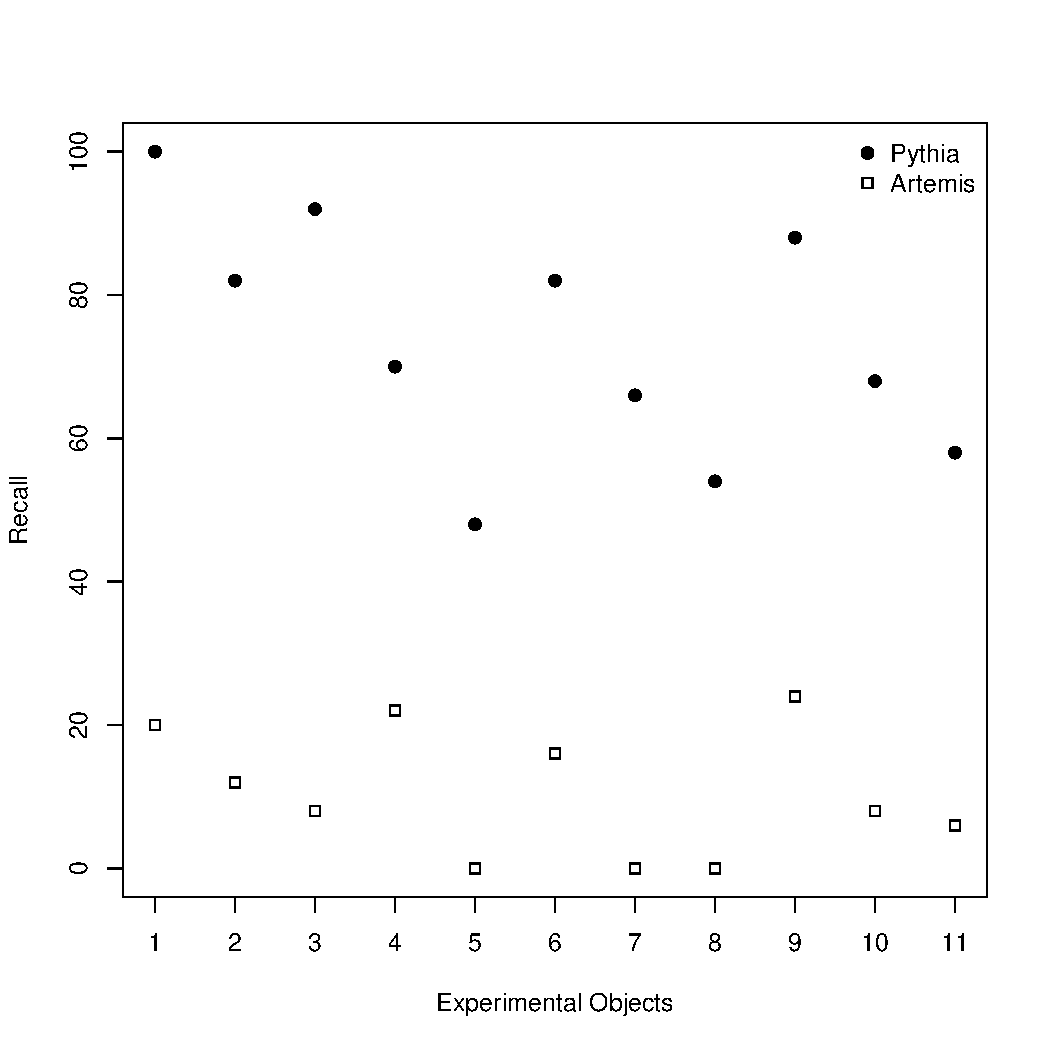
\includegraphics[width=0.9\hsize]{r-scripts/recall}
%  \mycaption{Recall of \tool and \artemis in detecting faults.}
%  \vspace{-0.1in} 
%  \label{Fig:recall-graph}
%\end{figure}

The table also shows that on average 32\% percent of the injected faults (ranges from 15--73\%) are detected by function-level test cases, but not by our DOM event-based test cases. This shows that a considerable number of faults do not propagate to observable DOM states, and thus cannot be captured by DOM-level event-based tests. 
For example in SimpleCart application (ID 10), if we mutate the mathematical operation that is responsible for computing the total amount of purchased items, the resulting error is not captured by event-based tests as the fault involves internal computations only. However, the fault is detected by a function-level test that directly checks the returned value of the function.
This points to the importance of incorporating function-level tests in addition to event-based tests for \javascript web applications. We also observed that even when an event-based test case detects a \javascript fault, localizing the error to the corresponding \javascript code can be quite challenging. However, function-level tests pinpoint the  corresponding function when an assertion fails, making it easier to localize the fault. 
%For example, in SameGame (ID 1), the function \code{compactDown} is responsible for moving cells up on the board after clicking on a given cell. If the index of the global variable \code{board} array is mutated in \code{compactDown}, the event-based tests shows an incorrect \code{background} value of the \code{css} property on the corresponding DOM elements. However, tracing the fault back to the responsible function is difficult. Using function-level tests, we can easily spot the assertion that is failed after calling \code{compactDown} function (e.g., \code{equal(board[3][4], 1)} failed).    

\headbf{Comparison (RQ3)}
\figref{coverage-graph} shows the code coverage achieved by  both \tool and \artemis on the experimental objects running for the same amount of time, \ie 10 minutes.
%Note that while \artemis only generates DOM event tests, \tool generates both unit tests and DOM event tests. 
%We compare the statement coverage achieved by \tool with that achieved by \artemis. 
The test cases generated by \tool achieve 68.4\% coverage on average (ranging from 41--99\%), while \artemis achieves only 44.8\% coverage on average (ranging from 0--92\%).
Overall, the test cases generated by \tool achieve 53\% more coverage than \artemis, which points to the effectiveness of \tool in generating high coverage test cases. 
Further, as can be seen in the bar plot of \figref{coverage-graph}, for all the applications, the test cases generated by \tool achieve higher coverage than those generated by \artemis. 
This increase was more than 226\% in the case of Bunnyhunt (ID 5). %\ali{Is this true? Isn't the difference in ID 7 and ID 8 more?}
For two of the applications, NarrowDesign (ID 7) and JointLondon (id 8), \artemis was not able to complete the testing task within the allocated time of ten minutes.
Thus we let \artemis run for an extra 10 minutes for these applications (\ie 20 minutes in total). Even then, neither application completes under \artemis. 
%By reducing the iteration option, \artemis produces an output after 10 minutes, however, with considerably lower coverage rates of 30\% and 35\% for NarrowDesign (ID 7), and JointLondon (ID  8), respectively. %I calculated the results based on zero coverage for these two apps, not sure if mentioning 30 and 35% here is correct or not!   

\tabref{faultDetection-table} shows the precision and recall achieved by \tool and \artemis.
With respect to fault finding capability, unlike \artemis that detects only generic faults such as runtime exceptions and W3C HTML validation errors, \tool is able to accurately distinguish faults at the code-level and DOM-level through the test oracles it generates. Both tools achieve 100\% precision, however, \tool achieves five-fold higher recall (70\% on average) compared with \artemis, which achieves 12.8\% recall on average. %Thus, \tool achieves more than five-fold increase in recall over \artemis.   

\subsection{Threats to Validity} \label{Sec:threatsToValidity}
An external threat to the validity of our evaluation is the limited number of \javascript applications used to measure the effectiveness of our approach. We mitigated this threat by using web applications from various domains, code size, and functionality. Another threat concerns validating failed assertions through manual inspection that can be error-prone. To mitigate this threat, we carefully examine the code in which the assertion failed to make sure that the injected fault was indeed responsible for the assertion failure. Moreover, manual computation of the \javascript slices to measure precision and recall is a time intensive task done by the authors of the paper, and thus could be error-prone. However, we made every effort to mitigate this threat by precisely examining the application's code.

The regression faults we inject to evaluate the effectiveness of \tool may not be realistic. We mitigate this threat by injecting mutations that represent common \javascript applications faults, as well as using real-world web applications, and \selenium test cases written by developers.
%\subsection{Discussion} \label{Sec:discussion}
\begin{figure}[!t]
  \centering
  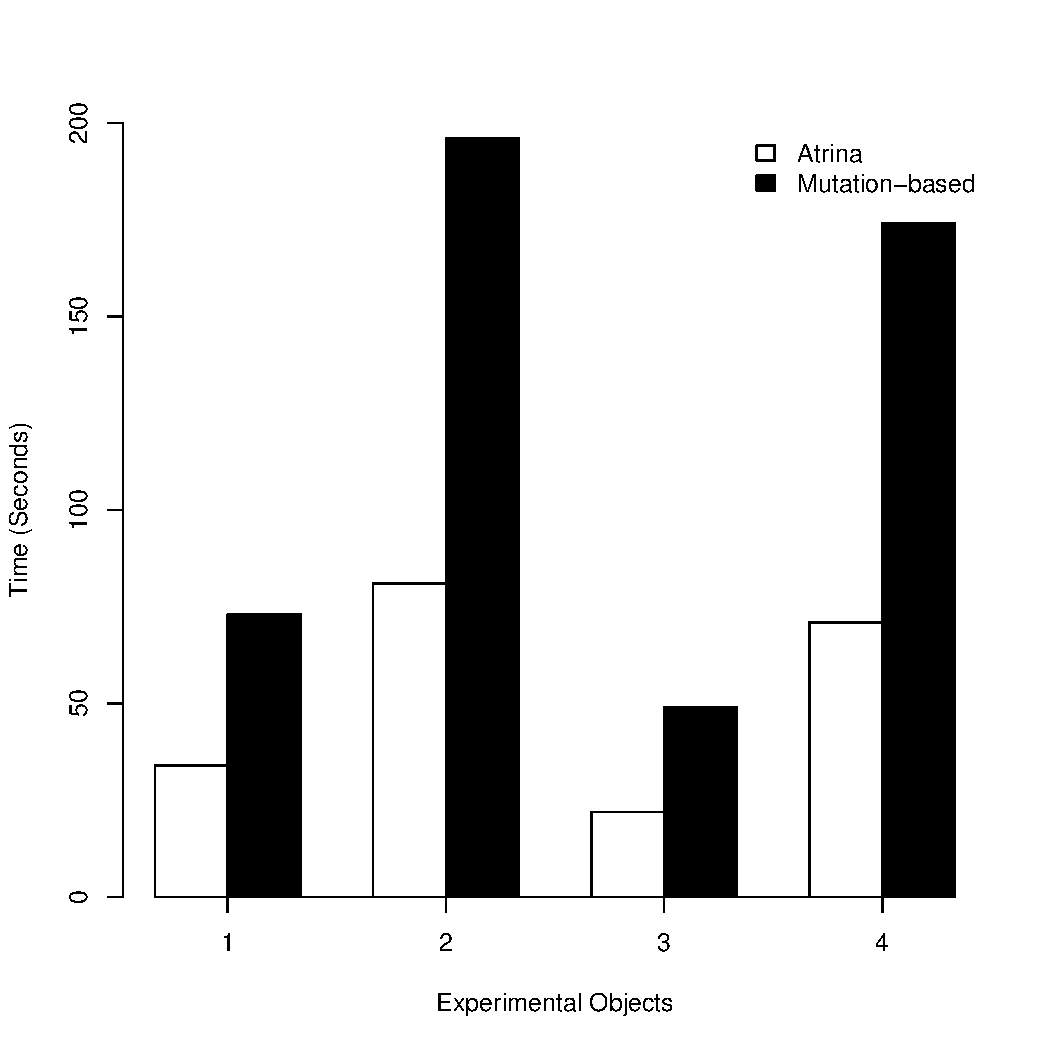
\includegraphics[width=0.7\hsize]{r-scripts/performance}
  \vspace{-0.18in}   
  \mycaption{Time overhead for each approach.}
  \vspace{-0.3in} 
  \label{Fig:performance}   
\end{figure}
% Moved time efficiency to results
%Moreover, this reiterates the known performance shortcomings of approaches that rely on mutant generation.
\headbf{Fault Masking} As we mentioned in \secref{explicitAssertions}, the concrete value of an entity in the computed backward slice can potentially be used as the expected value of the entity in explicit assertions to test the current version of the application.
The actual values of the related entities in the backward slice are correct unless there exists a masked fault which is concealed in the chain of computations and thus does not propagate to the checked state of the DOM element. However, we conjecture that fault masking rarely happens in \javascript web applications as it is more prevalent in programs with many small expressions whose results are stored in several intermediate values. We also observed no fault masking occurrence during the evaluation of \tool on seven \javascript applications used in this study.
\headbf{Limitations} The effectiveness of the generated assertions by \tool in terms of fault finding capability depends on the quality of human-written DOM-based test cases. If the DOM assertions contained in the DOM-based test suite check irrelevant information, the explicit assertions obtained by our tool will point to entities that may not be important from the tester's point of view. This can also negatively affect the fault finding capability of implicit assertions as they are indirectly inferred from the DOM-based assertions. Moreover, if the human-written test suite does not execute application's state with effective DOM elements, our tool is not able to infer effective candidate assertions.   


  

\section{Related Work} \label{Sec:related}


\headbf{Web application testing}
Marchetto and Tonella \cite{marchetto:search} propose a search-based algorithm for generating event-based sequences to test Ajax applications. 
Mesbah et al.  \cite{mesbah:tweb11} apply dynamic analysis to construct a model of the application's state space, from which event-based test cases are automatically generated. In subsequent work \cite{mesbah:tse12}, they propose generic and application-specific invariants as a form of automated soft oracles for testing \ajax applications.  Our earlier work, \jsart \cite{mirshokraie:icwe12},  automatically infers program invariants from \javascript execution traces and uses them as regression assertions in the code. 
Sen \etal \cite{sen:fse13} recently proposed a record and replay framework called Jalangi. It incorporates selective record-replay as well as shadow values and shadow execution to enable writing of heavy-weight dynamic analyses.
The framework is able to track generic faults such as \code{null} and \code{undefined} values as well as type inconsistencies in \javascript. 
Jensen \etal \cite{jensen:fse13} propose a technique to test the correctness of communication patterns between client and server in \ajax applications by incorporating server interface descriptions.
They construct server interface descriptions through an inference technique that can learn communication patterns from sample data.
Saxena \etal \cite{song:symb10} combine random test generation with the use of symbolic execution for systematically exploring a \javascript application's event space as well as its value space, for security testing.
Our work is different in two main aspects from these: (1) they all target the generation of event sequences at the DOM level, while we also generate unit tests at the \javascript code level, which enables us to cover more and find more faults,
and (2) they do not address the problem of test oracle generation and only check against soft oracles (e.g., invalid HTML). In contrast, we generate strong oracles that capture
application behaviours, and can detect a much wider range of faults.

Perhaps the most closely related work to ours is \artemis \cite{artzi:icse11}, which supports automated testing of \javascript applications.
\artemis considers the event-driven execution model of a \javascript application for feedback-directed testing.
In this paper, we quantitatively compare our approach with that of \artemis (Section \ref{Sec:evaluation}).

\headbf{Oracle generation} \label{Sec:oracleGen}
There has been limited work on oracle generation for testing. 
Fraser \etal \cite{fraser:tse12} propose $\mu$TE\-ST, which employs a mutant-based oracle generation technique.  It automatically generates unit tests for Java object-oriented classes by using a genetic algorithm to target mutations with high impact on the application's behaviour. They further identify~\cite{fraser:issta11} relevant pre-conditions on the test inputs and post-conditions on the outputs to ease human comprehension.
%\shabnam{differential test generation added for issta}
Differential test case generation approaches \cite{taneja:ase08, elbaum:tse09} are similar to mutation-based techniques in that they aim to generate test cases that show the difference between two versions of a program. However, mutation-based techniques such as ours, do not require two different versions of the application.
Rather, the generated differences are in the form of controllable mutations that can be used to generate test cases capable of detecting
regression faults in future versions of the program.
%\karthik{So what's the advantage of having the differences in the form of controllable mutations ?}
Staats \etal \cite{staats:icse12} address the problem of selecting oracle data,  which is formed as a subset of internal state variables as well as outputs for which the expected values are determined.
They apply mutation testing to produce oracles and rank the inferred oracles in terms of their fault finding capability.
This work is different from ours in that they merely focus on supporting the creation of test oracles by the programmer, rather than fully automating the process of test case generation. Further, (1) they do not target \javascript; 
(2) in addition to the code-level mutation analysis, we propose DOM-related mutations to capture error-prone \cite{Ocariza:esem2013} dynamic interactions of \javascript with the DOM.  



\section{Conclusions} \label{Sec:concs}
In this paper, we present an automated technique to generate unit-level assertions for the \javascript code. Given (1) a web application that highly interact with the DOM through the underlying \javascript code, and (2) a DOM-based test suite, we make use of the human-written DOM-based test cases to generate effective assertions that can capture regression faults in the \javascript code. We implemented our approach in an open-source tool called \tool. We empirically evaluated \tool on four web applications. The results show that our approach (1) is accurate in mapping the assertions to the\javascript code, (2) is effective in detecting injected regression faults (62\% on average), (3) outperforms human-written DOM-based assertions in terms of fault finding capability by 37\% on average, and (4) generates unit assertions that are more effective (29\% on average) than those produced by mutation-based technique.

% use section* for acknowledgement
%\section*{Acknowledgment}


%\balance

\bibliographystyle{abbrv}
\bibliography{../biblio}



% that's all folks
\end{document}